\documentclass[parskip=full]{scrartcl}

\pdfoutput=1

\title{Small Data Oversampling  \\ \LARGE{Improving small data prediction accuracy using the Geometric SMOTE algorithm}}

\author{
	Georgios Douzas\(^{1}\), Fernando Bacao\(^{1*}\), Maria Lechleitner\(^{1}\) 
	\\
	\small{\(^{1}\)NOVA Information Management School, Universidade Nova de Lisboa}
	\\
	\small{*Corresponding Author}
	\\
	\\
	\small{Postal Address: NOVA Information Management School, Campus de Campolide, 1070-312 Lisboa, Portugal}
	\\
	\small{Telephone: +351 21 382 8610}
}

\usepackage{breakcites}
\usepackage{float}
\usepackage{graphicx}
\usepackage{geometry}
\usepackage[colorinlistoftodos]{todonotes}
\geometry{
	a4paper,
	total={170mm,257mm},
	left=18mm,
	right=18mm,
	top=8mm,
}
\usepackage{amsmath}
\newcommand{\inlineeqnum}{\refstepcounter{equation}~~\mbox{(\theequation)}}
\usepackage{enumitem}
\usepackage[ruled,vlined]{algorithm2e}
\usepackage{booktabs}
\usepackage{pgfplotstable}
\pgfplotsset{compat=1.14}
\usepackage{longtable}
\usepackage{tabu}
\usepackage{hyperref}
\date{}

\begin{document}

\maketitle

\begin{abstract}
Many small data set learning tasks are limited due to an incomplete data 
structure where information for decision making is missing. This research aims 
to improve predictive performance by artificially adding samples in the 
pre-processing phase of the data analysis process. Based on the oversampling 
technique G-SMOTE, the new application of the algorithm generates artificial 
samples to enhance crisp data structures. The results of the experiments show a 
significant improvement on the prediction capability when comparing with other 
oversampling techniques such as SMOTE and random oversampling. 
\end{abstract}

\section{Introduction}
One of the key problems in supervised learning is the insufficient size of data
sets \cite{Niyogi.1998}. The limited availability of training sample sets can be
caused by different factors. First, data is becoming an increasingly expensive 
resource \cite{Li.2007} as the process to retain data is getting more complex 
due to strict privacy regulations such as the General Data Protection 
Regulation (GDPR) \cite{EuropeanCommission.2019}. Additionally, the small 
dataset problem can be found in numerous industries where organizations simply 
do not have access to a reasonable amount of data, for example: manufacturing 
industries are usually dealing with small data in early stages of product 
developments; health care organizations have to work with different kinds of 
rare diseases, where very few records around the world are available; and in 
financial industries, fraud detection is an important issue with only few 
examples for cases of violence \cite{AbdulLateh.2017}.

A sufficient training sample set is one of the basic assumptions in Machine
Learning \cite{Ivanescu.2006}. However, in the context of computational learning
theory, small sample size is one of the most frequent difficulties among
measurement error, model fitting and characteristics of predictors
\cite{AbdulLateh.2017}. The issue with small datasets is that they do not 
provide an unbiased representation of reality due to a loose data structure 
with many information gaps. This lack of learning information negatively 
impacts the performance of the machine learning algorithms \cite{Lin.2018}. 
Consequently, the knowledge gained from prediction models trained with small 
sample sizes is considered unreliable as well as imprecise and does not lead to 
a robust classification performance \cite{AbdulLateh.2017}.

Considering the size of data there are two types of measurements: first, the 
insufficiency of data belonging to one class (imbalance data problem); and 
second, the insufficiency in the whole data (small dataset problem) 
\cite{Sezer.2014}. In both cases, a small training sample set does not provide 
enough information to a machine learning model to obtain a stable learning 
accuracy \cite{Tsai.2008}. A theoretical explanation of “small” can be found in 
statistical learning theory by Vapnik. A sample size is defined as small, if 
the ratio between the number of training samples and Vapnik-Chervonenkis (VC) 
dimensions is less than 20. Where VC dimensions are determined as the maximum 
number of vectors that can be separated into two classes in all possible ways 
by a set of functions \cite{Vapnik.2008}. 

\begin{figure}[H]
	\centering
	\includegraphics[width=0.6\linewidth]{"./resources/vc_dimension"}
	\caption{Example of VC Dimension \cite{Vapnik.2008}}
	\label{fig:vc-dimension}
\end{figure}

In the figure presented above, the VC dimension is equal to 3, since the lines
in the graph can shatter three vectors (see graphic to the left). As it is
demonstrated in the graph on the right side, the vectors z{\tiny 2} and z{\tiny
4} cannot be separated by a line from the vectors z{\tiny 1} and z{\tiny 3}
\cite{Vapnik.2008}.

Under-representation of observations in the sample set can be solved in 
different ways. The use of synthetic data derived from existing (real) 
observations is a promising approach to the problem \cite{Sezer.2014}. As a 
result, techniques to artificially add information by extending the sample size 
and eventually improving classification results of the algorithms can translate 
into significant improvements in many application domains. However, it is 
important to consider that virtual data samples are not necessarily 
representatives of the population, as they are artificially created. Taking 
this into consideration, the challenge in artificial data generation is to 
create data which extends the observed data without creating noise 
\cite{Li.2006}. 

\begin{figure}[H]
	\centering
	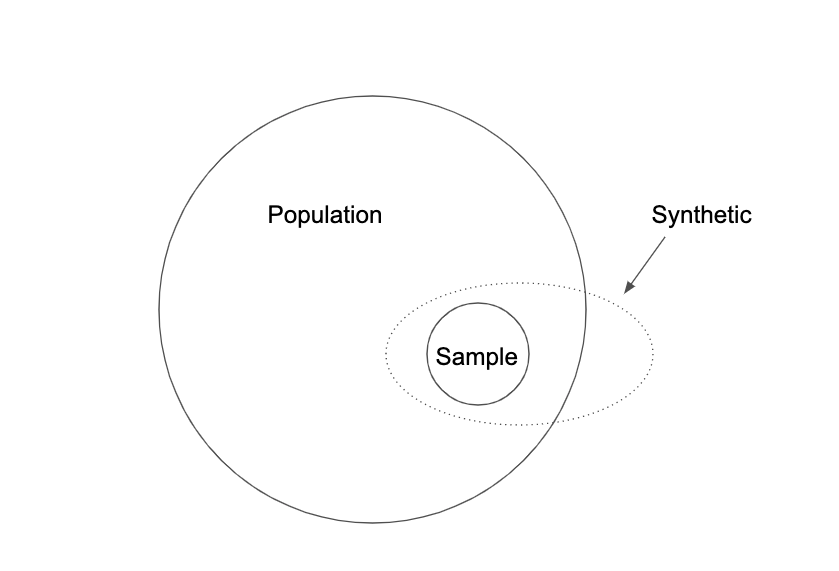
\includegraphics[width=0.35\linewidth]{./Resources/relationship}
	\caption{Relationship between population, actual data and virtual data \cite{Li.2006}}
	\label{fig:relationship}
\end{figure}

The next sections will describe an effective way to tackle this problem. First, 
the previously studied solutions are reviewed. Second, a detailed description 
of the proposed method is presented. This is followed by the research 
methodology and the experimental results in Chapter 4 and 5. Finally, the paper 
is concluded with an analysis of the experiments in Section 6.

\section{Related Work}
Several data pre-processing methods to handle small dataset problems have been
presented by the research community. In this section, the most important
approaches are reviewed and the state-of-the-art to improve small dataset
learning is reported. We start by presenting fuzzy theories, which have 
historically been the most used approach to mitigate the small dataset problem. 
Next, we look at resampling mechanisms, which mainly consist of bootstrapping 
techniques, and finally, we review oversampling techniques that can be a 
valuable option to increase the sample size in small datasets.

\subsection{Fuzzy Theories}

In order to build an accurate prediction model, a large sample of the 
population is required to train the model. One of the most effective methods to 
improve the learning performance of prediction models is artificial sample 
generation. It is proven that the accuracy of the learning algorithm is 
improved, when increasing the sample size of training sets 
\cite{AbdulLateh.2017}. Thus, the objective is to fill the gaps between 
observations (information gaps) with synthetic samples that are derived from 
the original population to feed the algorithm with a more complete 
representation of the reality.

\begin{figure}[H]
	\centering
	\includegraphics[width=0.6\linewidth]{"./Resources/small_data_distribution"}
	\caption{Distribution of a small dataset}
	\label{fig:small-data-distribution}
\end{figure}

Many techniques presented in the literature are based on fuzzy theories
\cite{AbdulLateh.2017}. The fuzzy set theory provides a strict mathematical
framework to generalize the classical notion of a dataset. It gives a wider
scope of applicability, especially in the fields of information processing and
pattern classification \cite{Zimmermann.2010}. Based on this concept, several
methods have emerged in the last decade to estimate or approximate functions
which are generating more samples for sparse training sets.

The fundamental concept of artificially creating data is called Virtual Sample 
Generation (VSG) and was originally proposed by \cite{Niyogi.1998}. The idea is 
to create additional examples based on the current set of real-life examples by 
using prior information gained from the available data. The introduction of 
virtual examples expands the effective training set size and can therefore help 
to mitigate the learning problem. \cite{Niyogi.1998} proved that the process of 
creating artificial samples is mathematically equivalent to incorporating prior 
knowledge. They demonstrate the concept on object recognition by mathematically 
transforming the views of 3D-objects. These new views are called ‘virtual 
samples’ and its application extends information and results in successful 
generalization. 

Based on this theory, several closely related studies were developed for
manufacturing environments. The first method to overcome scheduling problems due
to the lack of data in early stages of manufacturing systems was the creation of
a Functional Virtual Population (FVP) \cite{Li.2003}. The idea is to
create a number of virtual samples within of a newly defined domain range. The
method involves a highly manual process, however, the application of FVP
dramatically improved the classification accuracy of a Neural Network. 

In 2004, the idea of fuzzifying information to extend a small dataset was used 
to develop the Diffusion-Neural-Network (DNN) method \cite{Huang.2004}. I 
combines the principle of information diffusion by \cite{Huang.1997} with 
traditional Neural Networks to estimate functions. The information diffusion 
method partially fills the information gaps by using fuzzy theories to 
represent the similarities between samples and subsequently derive new samples. 

The researchers \cite{Li.2006b} further examined possible methods to learn
scheduling knowledge with rare data in early stages of manufacturing systems.
They developed a new data fuzzification technique called mega-fuzzification and
combined it with a data trend estimation procedure to systematically expand the
small dataset. The method fuzzifies the dataset as a whole and expands it in
consideration of a previously defined data trend. The results of this study 
show high learning accuracy and denote the method as a reliable and applicable 
approach in the business marketplace. However, the difficulty in establishing 
the domain ranges and the lack of a theoretical basis explain its lack of 
popularity and limited interest. 

In order to fully fill the information gaps, a technique which diffuses the
sample set one for one was introduced by \cite{Li.2007}. To avoid the
over-estimation, their concept is to combine data trend estimation with a mega
diffusion technique to estimate the domain range. The method is called
Mega-Trend-Diffusion (MTD) and diffuses a set of data instead of each sample
individually. For example, two samples m and n (Figure 4) are diffused
simultaneously into one function with their borders $\mathit{a}$ and 
$\mathit{b}$. To estimate $\mathit{a}$ and $\mathit{b}$, the algorithm takes 
the minimum and maximum values of the dataset and counts the number of data 
points which are smaller or greater than the average of the values. This takes 
the skewness in the distribution of the data and the domain range into 
consideration when calculating new samples. The triangular shape of figure 4 
represents the membership function which shows the similarities between 
samples. $\mathit{M}$ and $\mathit{n}$ are the samples and their heights are 
the possible values of the membership function.

\begin{figure}[H]
	\centering
	\includegraphics[width=0.7\linewidth]{"./Resources/mtd_function"}
	\caption{MTD function}
	\label{fig:mtd-function}
\end{figure}

After estimating the domain range between $\mathit{a}$ and $\mathit{b}$, 
samples are randomly produced within this area by using a common diffusion 
function. The artificial samples are then trained with a Back-propagation 
Neural Network (BPNN) like \cite{Huang.2004} originally proposed. This 
technique is seen as an improvement of DNN and was initially developed to 
improve early flexible manufacturing system scheduling accuracy. In further 
research, MTD is widely used as a synthetic sample generation method and is 
recognized as an effective way to deal with small dataset problems 
\cite{AbdulLateh.2017}. However, MTD only considers the data for independent 
attributes and does not deal with their relationships. 

A genetic algorithm based virtual sample generation (GABVSG) was also proposed. 
The method takes the relationship among the attributes into account and 
explores the integrated effects of attributes instead of dealing with them 
individually. This algorithm is performed in three steps: Samples are randomly 
selected to determine the range of each attribute by using MTD functions. Next, 
a Genetic Algorithm is applied to find the most feasible virtual samples. 
Finally, the average error of these new samples is calculated. The results 
outperformed the ones using MTD and also showed better performance in 
prediction than in case of no generation of synthetic samples \cite{Li.2014}.

The above presented fuzzy-based algorithms are limited on numerical attributes. 
When the dataset contains nominal features, resampling mechanisms have to be 
considered such as Bootstrap. Although it is possible to transform nominal 
values into binary ones, the relationship between the values of the attributes 
would get lost \cite{Tsai.2008}. 

\subsection{Resampling Mechanism}

An alternative approach to fuzzy theories is a statistical method called the 
Bootstrapping procedure (BP), which is the most well-known artificial sample 
generation method \cite{AbdulLateh.2017}. The main difference to the previously 
presented techniques is that BP creates new training sets by resampling 
instances from the measured data with replacement. This means that after a data 
point is selected for a new sample set, it is still available for further 
selection \cite{Efron.1993}. It allows the algorithms to use the same sample 
more than one time to gradually revise the identified patterns in order to 
improve predictive accuracy. Although this can double the number of 
observations from the training sets (shown in Fig. 5.a.), Bootstrapping can 
cause overfitting when applied to small data because it only represents a few 
observations. Also, since the amount of information provided by small data is 
minimal, any missing observations in the new, bootstrapped training sets are a 
loss of valuable information (see Fig. 5.b.). In general, the amount of 
information does not increase by performing Bootstrapping, because the 
increased information is the same information provided by the same observations 
\cite{Li.2018}. As a result, it is seen as a unfavourable technique, because it 
aims to increase the amount of observations used for training, rather than 
filling the information gaps with missing data \cite{Tsai.2015}. However, 
\cite{Ivanescu.2006} applied BP in batch process industries where they proofed 
that the bootstrapping procedure can indeed solve the limited data problem.

\begin{figure}[H]
	\centering
	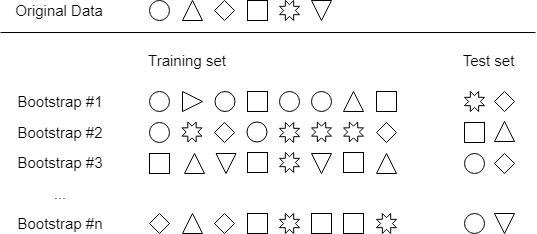
\includegraphics[width=0.9\linewidth]{resources/bootstrapping_example}
	\caption{Example of bootstrapping sets, where a) is the set for which the 
	observations are doubled and b) are two possible sets}
	\label{fig:bootstrappingexample}
\end{figure}

In further studies of \cite{Tsai.2008} and \cite{Chao.2011}, the bootstrap 
procedure was applied to actually generate virtual samples in order to fill the 
information gaps. Instead of resampling observations, they execute the BP once 
for each input factor which results in a newly shuffled training set. After 
generating new instances, they are combined with the original dataset to train 
a Neural Network. The results show that this method significantly decreases the 
prediction error rate in modelling manufacturing systems as well as in the 
prediction to radiotherapy of bladder cancer cells.

\subsection{Oversampling Techniques}

A different approach to fill information gaps is synthetic oversampling of the
training set. Oversampling is an artificial data generation strategy originally
developed in the context of machine learning to mitigate the imbalanced 
learning problem. The origin of oversampling comes from a different research 
community which is more related to machine learning techniques. Although 
oversampling, fuzzy and resampling approaches are aiming to solve a similar 
problem, it seems that these communities have had very few contact so far. In 
Imbalanced Learning, the classes of the given dataset are significantly skewed 
in a sense that there is a difference between examples of different classes. 
This means, that the dataset has a large number of observations in one class 
and a very small number of observations in the other class or classes. This 
constitutes a problem for the algorithm to learn and is aimed to be solved in 
the data pre-processing phase. In practice, the imbalanced dataset problem is 
are very common issue in Supervised Learning. Especially, in the fields of 
fraud detection, product categorization and disease diagnosis an imbalanced 
dataset is the norm rather than the exception \cite{He.2013}. 

\subsubsection{SMOTE}

There are several methods presented in the literature to tackle this problem.
One of the first and most popular methods is the synthetic minority
over-sampling technique (SMOTE). SMOTE works on the idea of k-nearest
neighbors. It generates synthetic data around vectors between the minority
class instances and their nearest neighbors \cite{Chawla.2002}. A visual
representation of the concept can be found in figure 5.

\begin{figure}[H]
	\centering
	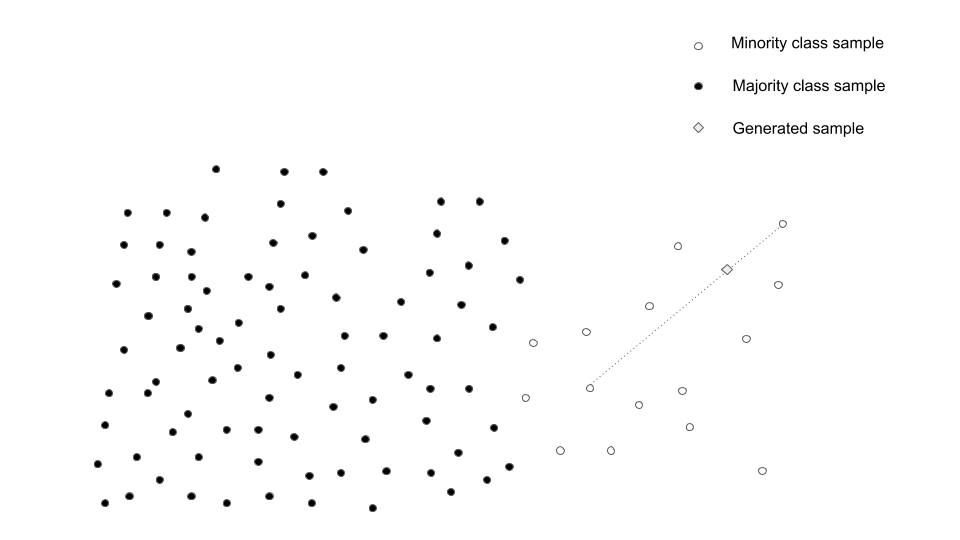
\includegraphics[width=0.5\linewidth]{./Resources/smote}
	\caption{Concept of SMOTE}
	\label{fig:smote}
\end{figure}

The algorithm is considered as a standard framework for pre-processing
imbalanced datasets due to its simplicity and as well as its robustness.
Numerous variations of SMOTE have been developed which declares SMOTE as the
foundation of synthetic sample generation when it comes to imbalanced
classification problems \cite{Fernandez.2018}. However, the algorithm faces some
limitations when it comes to the sample generation process. In practice, the
separation between majority and minority class clusters is often not clearly
definable. Thus, noisy samples may be generated when a minority sample lies in
the region of the majority classes. Figure 7 presents a scenario where a
minority instance is generated within the majority region (noisy sample).

\begin{figure}[H]
	\centering
	\includegraphics[width=0.6\linewidth]{"./resources/noisy_examples"}
	\caption{Generation of noisy examples}
	\label{fig:noisy-examples}
\end{figure}

Furthermore, redundant instances may be generated within dense minority regions.
They do not add any relevant information to the classifier and may lead to
overfitting. Figure 8 demonstrates an example where a minority class instance is
generated in a dense minority class. This new observation belongs to the same
dense cluster as the original and is therefore less useful. 

\begin{figure}[H]
	\centering
	\includegraphics[width=0.6\linewidth]{"./Resources/redundant_examples"}
	\caption{Generation of redundant examples}
	\label{fig:redundant-examples}
\end{figure}

Although SMOTE is recognized as a oversampling technique for imbalanced
datasets, it is also used for solving the small dataset problem \cite{Li.2018}.
By performing simple adjustments in the algorithm, it successfully fills the
information gaps with synthetic samples. However, it did not achieve the best
results within the study.

\subsubsection{G-SMOTE}

A the novel data generation procedure Geometric SMOTE (G-SMOTE) has been 
presented with the objective to improve the above mentioned limitations of the 
SMOTE algorithm \cite{Douzas.2019b}. G-SMOTE is an extension of SMOTE can be 
seen as a substitute. The main difference to SMOTE is that the novel method 
significantly broadens the options for data generation and prevents the 
creation of noise. Instead of connecting the minority sample and its nearest 
neighbour with a line segment (hypersphere), the instances are generated in a 
geometrical region (hyper-spheroid) around the minority sample. Furthermore, 
G-SMOTE is designed to avoid the generation of noisy samples by some 
restrictions in the selection strategy. Figure 8 demonstrated the distribution 
of artificially created samples by SMOTE versus G-SMOTE. With an increased 
number of k neighbors, SMOTE tends to generate noisy samples, whereas Geometric 
SMOTE avoids this scenario.

\begin{figure}[H]
	\centering
	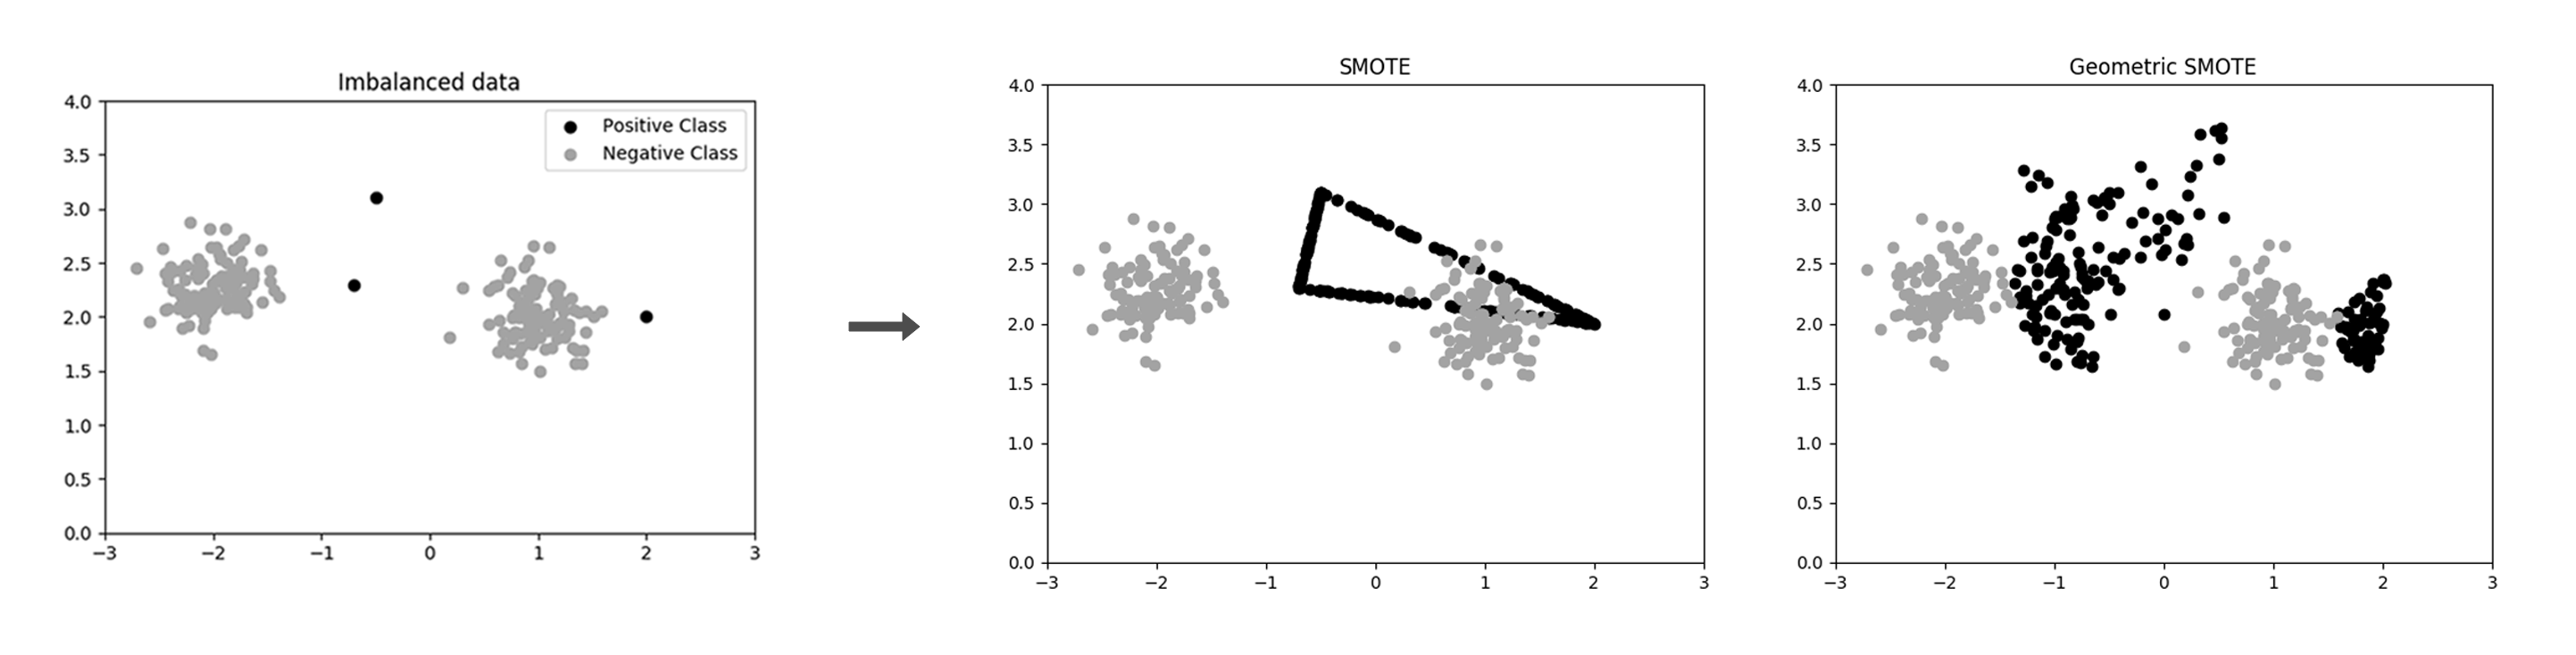
\includegraphics[width=0.8\linewidth]{resources/smote_vs_gsmote}
	\caption{SMOTE versus G-SMOTE \cite{Douzas.2019}}
	\label{fig:smotevsgsmote}
\end{figure}

These modifications of SMOTE proof their refinement in experiments with 69 
imbalanced datasets and four classifiers such as Logistic Regression (LR), 
K-Nearest Neighbours (KNN), Decision Tree (DT) and Gradient Boosting (GBC). The 
results show that G-SMOTE is outperforming SMOTE, Random Oversampling and the 
case of no oversampling, across all datasets, classifiers and performance 
metrics.    

Various methods to deal with small datasets as well as small representation 
within a class label have been presented in this section. It has been proven, 
that all cases with artificially increased sample size seem to enhance the 
prediction performance of the conventional classifier. Thus, we can conclude 
that data pre-processing of a small or imbalanced dataset by increasing the 
sample size is an important task in the area of Machine Learning 
\cite{Ruparel.2013}. However, most of the studied methods are associated with a 
lot of limitations and are hard to understand. In practice, an application of 
these methods has still been challenging \cite{Sezer.2014}. As a result, we 
propose a different approach to overcome the issues sourced form the absence of 
data and provide a framework for an easy implementation of the algorithm.

\section{Proposed Method}

In the following section, we propose G-SMOTE as novel data generation procedure 
for small sample sets. Originally developed for imbalanced datasets, we 
slightly adapt the algorithm to not only increase the minority class, but the 
entire sample set independent from class occurrences. 

\subsection{G-SMOTE for small data}

As mentioned above, the G-SMOTE algorithm randomly generates artificial data 
within a geometrical region of the input space. The size of this area is 
derived from the distance of the selected sample to the nearest neighbour, 
whereas the shape is determined by the hyperparameters truncation factor and 
deformation factor. Additionally, the direction of the new input area is 
defined by the selection strategy of G-SMOTE. The main concept can be adapted 
from the original method. However, the selection strategy requires some minor 
adjustments for the small dataset problem which will be described in the 
following.

The selection strategy $\alpha$\textsubscript{sel} determines the data points 
of the $\mathit{k}$ nearest neighbors. This mechanism allows the positive or 
negative class area to expand into a direction where it prevents the algorithm 
from creating noisy samples. In G-SMOTE for small data both classes are 
selected in two individual runs to introduce new observations. In the first 
run, a random sample called x\textsubscript{surface} is selected which belongs 
to the positive class. Similarly, x\textsubscript{surface} is assigned to the 
negative class samples in the second run. Both runs are based on the defined 
selection strategy where $\alpha$\textsubscript{sel} can have three different 
values: positive class selection S\textsubscript{pos}, negative class selection 
S\textsubscript{neg} and combined selection S\textsubscript{com}. We describe 
the cases referring to first run of randomly selecting a positive sample. In 
the second run, a negative class example is randomly chosen and the process is 
repeated reversely. 

\begin{enumerate}[label=($\alph*$)]

\item Positive class selection

With the hyperparameter selection\_strategy = 'positive', a second positive 
class sample is selected as one of the k nearest neighbors. This indicates that 
the selection strategy is based only on the positive class and works like the 
selection strategy of SMOTE. As SMOTE may lead to the generation of data 
penetrating the opposite class area, this drawback also applies on the 
selection strategy here.

\begin{figure}[H]
	\centering
	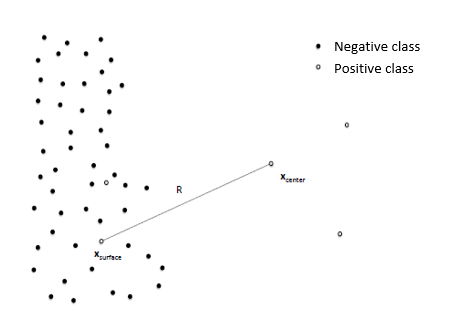
\includegraphics[width=0.6\linewidth]{resources/positive_class_selection_strategy}
	\caption{Example of positive class selection strategy: A positive class 
	instance is defined as the center and one of its $\mathit{k = 4}$ positive 
	class nearest neighbors is selected as the surface point. The radius 
	$\mathit{R}$ is equal to the distance of these instances.}
	\label{fig:positiveclassselectionstrategy}
\end{figure}

\item Negative class selection

When selection\_strategy = 'negative', the second sample is its nearest 
negative class neighbor. This scenario prevents the algorithm from creating 
noisy samples. More specifically, as the radius is drawn from the selected 
positive class instance to the nearest neighbour of the negative class, it does 
not allow the data generation mechanism to penetrate the opposite area.

\begin{figure}[H]
	\centering
	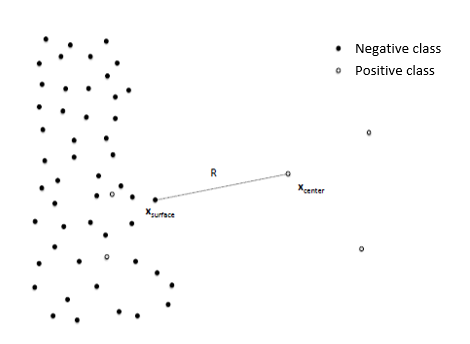
\includegraphics[width=0.6\linewidth]{resources/negative_class_selection_strategy}
	\caption{Example of negative class selection strategy: A positive class 
	instance is defined as the center and its closest negative class neighbor 
	is selected as the surface point. The radius R is defined to be equal to 
	the distance of these instances.}
	\label{fig:negativeclassselectionstrategy}
\end{figure}

\item Combined selection

The combined selection strategy initially applies the positive and negative 
selection strategies. Once x\textsubscript{pos} and x\textsubscript{neg} are 
identified, the point with the minimum distance to the center 
x\textsubscript{center} is defined as the surface point 
x\textsubscript{surface}. Figure 11 presents an example when 
x\textsubscript{surface} is identified as a negative class instance.

\begin{figure}[H]
	\centering
	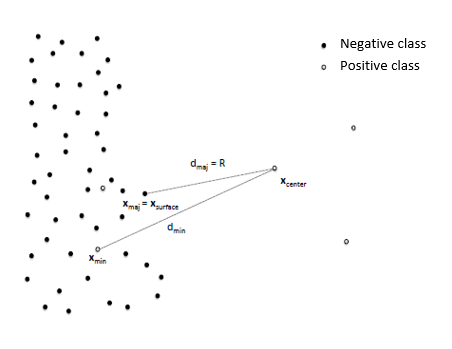
\includegraphics[width=0.6\linewidth]{resources/combined_class_selection_strategy}
	\caption{The closest point to the center positive class sample is 
	identified as the surface point since it is closer to the center than the 
	selected instance from the k nearest positive class neighbors of the 
	center.}
	\label{fig:combinedclassselectionstrategy}
\end{figure}
\todo{graphic has to be changed}

\end{enumerate}

%More adjustments?

\subsection{Adapted G-SMOTE algorithm}

The adapted G-SMOTE algorithm can be generally described in the following steps:

\begin{enumerate}
	\item 
	An empty set S\textsubscript{gen} is initialized
	\item 
	The S\textsubscript{pos} elements are shuffled and the process described 
	below is repeated $\mathit{N}$ times until $\mathit{N}$ artificial points 
	have been generated.
	\item 
	A positive class instance x\textsubscript{center} is selected as the center 
	of the geometric region.
	\item 
	Depending on the values of $\alpha$\textsubscript{sel} (positive, negative 
	or both), this step results in a randomly selected sample 
	x\textsubscript{surface} which belongs either to the positive or negative 
	sample set
	\item 
	A random point e\textsubscript{sphere} is generated on the surface of a 
	unit hypersphere centered at the origin of the input space. This point is 
	transformed to a randomly generated point x\textsubscript{gen} inside the 
	unit hypersphere. 
	\item 
	The geometrical transformations are applied to define the admissible area 
	for x\textsubscript{gen}. These are defined as truncation 
	$\alpha$\textsubscript{trunc}, which defines the subarea of the hypersphere 
	and deform $\alpha$\textsubscript{def}, which deforms the hypersphere. 
	
	\begin{enumerate}[label=($\alph*$)]
		\item 
		The truncation factor $\alpha$\textsubscript{trunc} defines the degree 
		of truncation that is applied to the geometric area and can be 
		specified between zero and one, where truncation\_factor=0.0 
		corresponds to a circle and truncation\_factor=1.0 becomes a 
		half-hypersphere around the selected sample. 
		
		\item 
		The formation of the area is defined by the so-called deformation 
		factor. If the parameter of the deformation factor is equal to 0, the 
		data generation area obtains a circle. On the opposite, if the 
		parameter is set to 1, the area deforms to a line segment. 
		For a graphical example of these hyperparameters the reader is referred 
		to (Douzas, 2019).
	\end{enumerate}

	\item 
	The generated point x\textsubscript{gen} is translated
	\item 
	x\textsubscript{gen} is added to S\textsubscript{gen}
	\item 
	Once this process is repeated $\mathit{N}$ times: S\textsubscript{neg} 
	elements are shuffled, a negative class instance is selected as 
	x\textsubscript{center} and the algorithm starts again with step 4 until 
	$\mathit{N}$ negative samples are introduced
\end{enumerate}

\section{Research Methodology}

The main objective of this work is to compare G-SMOTE with other oversampling 
techniques when it comes to the small dataset problem. Therefore, we use a 
variety of datasets, evaluation measures and classifiers to evaluate the 
performance. A description of this set-up, the experimental procedure as well 
as the software implementation is provided in the following section.

\subsubsection{Experimental Data}

Ten datasets are used to test the performance of G-SMOTE which are retrieved 
from UCI Machine Learning Repository \cite{Dua.2019}. The focus on the 
selection of the data lies on binary classification problems with a highly 
balanced distribution of the two classes. In order to assure generalizability 
of the results, the data sets include different topics such as health care, 
finance, business and physics as well as different sample sizes. Details of the 
datasets are presented in the following table:

\begin{table}[H]
	\centering
	\begin{tabular}{|l|l|l|l|}
		\hline
		\textbf{Dataset} & \textbf{Number of samples} & \textbf{Number of 
		attributes} & \textbf{Area} \\
		\hline
		Arcene & 900 & 10.000 & Health Care \\
		\hline
		Audit & 776 & 18 & Business \\
		\hline
		Banknote Authentication & 1.372 & 5 & Finance \\
		\hline
		Spambase & 4.610 & 57 & Business\\
		\hline
		Breast Cancer & 699 & 10 & Health Care\\
		\hline
		Indian Liver Patient & 583 & 10 & Health Care\\
		\hline
		Ionosphere & 351 & 34 & Physics\\
		\hline
		MAGIC Gamma Telescope & 19.020 & 11 & Physics\\
		\hline
		Musk & 6.598 & 168 & Physics\\
		\hline
		Parkinsons & 197 & 23 & Health Care\\
		\hline
	\end{tabular}
\caption{\label{tab:datasets}Description of the datasets}
\end{table}

\subsubsection{Evaluation Measures}

To evaluate the performance of G-SMOTE, the experiment includes two different 
measures. First, accuracy is used as one of the most common metrics for 
evaluating classification models \cite{M.2015}. Informally, accuracy measures 
the ratio of correct predictions over the total number of instances evaluated. 
The accuracy metric can be stated mathematically as

\[Accuracy = \frac{TP + TN}{TP + TN + FP + FN}\],

where $\mathit{TP/TN}$ denote the number of correctly classified positive as 
well as negative instances and $\mathit{FP/FN}$ denote the number of 
misclassified negative and positive instances, respectively. The accuracy 
metric might be negligible for datasets with a significant disparity between 
the number of positive and negative label. As pointed out by many studies, 
accuracy has limitations in the discrimination process since rare classes have 
only few impacts on the measure compared to majority classes. To make sure the 
accuracies of the two classes stay relatively balanced, we include the 
geometric mean as a second measure. G-Mean measures the trade-off between 
sensitivity (true positive rate) and specificity (true negative rate) by the 
following:

\[G-Mean = \sqrt{sensitivity \times specificity} = \sqrt{\dfrac{TP}{TP + FN} 
\times \dfrac{TN}{TN + FP}}\]

The objective of both measures is to be maximized since a classifier is 
performing well if it provides high classification accuracy and a high ratio of 
positive and negative accuracy \cite{Han.2012}. 

\subsubsection{Machine Learning Algorithms}

The experiment is conducted with several classifiers to make sure the results 
are not dependent on the machine learning algorithm. We use the following four 
classifiers: Logistic Regression (LR) \cite{McCullagh.2019}, K-Nearest 
Neighbors (KNN) \cite{Cover.1967}, Decision Tree (DT) \cite{Salzberg.1994} and 
Gradient Boosting (GBC) \cite{Friedman.2001}. Descriptions of these algorithms 
are provided in the given studies.

\subsubsection{Experimental Procedure}

The main concept of the experimental procedure is to randomly under-sample 
medium to big sized datasets, increase them artificially and eventually compare 
the results with the original dataset which is considered to be the benchmark. 
This method allows us to directly compare the quality of the artificial 
generated sample set with the observed data. In order to evaluate if the 
proposed method can improve artificial data generation, we compare G-SMOTE with 
SMOTE, random oversampling and no oversampling. 

We use $\mathit{k}$-fold cross-validation with $\mathit{k = 5}$ as a technique 
for assessing the performance of the models for each combination of oversampler 
and classifiers. The dataset $\mathit{D}$ is randomly split into $\mathit{k}$ 
subsets (folds) $\mathit{D_1, D_2, … D_k}$ of approximately equal size. Each 
fold is used as a validation set and the remaining folds are used to train the 
model with $\mathit{k}$ iterations. This procedure is repeated until each 
$\mathit{k}$ have been used as a validation set \cite{Han.2012}. Based on this 
technique, the experiment is conducted in the following steps within one 
iteration:

\begin{enumerate}
	\item 
	Splitting dataset into $\mathit{k}$-fold cross-validation sets where 
	$\mathit{k = 5}$
	\item 
	Undersampling $\mathit{k - 1}$ folds such that the class frequency remains 
	the same as the original
	\item 
	Synthetic oversampling of $\mathit{k - 1}$ folds to the original size of 
	the dataset (class ratio remains the same) with G-SMOTE, SMOTE, Random 
	Oversampling and undersampled data (No oversampling)
	\item 
	Training the model with the classifiers LR, KNN, DT and GBC
	\item 
	Testing the model with the remaining, original fold
	\item 
	Computation of results
\end{enumerate}	

This procedure is repeated three times and the highest cross validation score 
for each combination of dataset, classifier, oversampler and evaluation metric 
is reported. The presented numbers are the average values computed from the 
three runs. In order to confirm the statistical significance of the 
experimental results, the Friedman test \cite{Sheldon.1996} as well as the 
Holms test \cite{JanezDemsar.2006} are applied. The Friedman test is a 
non-parametric procedure to test hypothesis an ordinal scaled variables. 
Additionally, it can also be applied with interval data when normality and 
homogeneity assumption does not hold. We use the Friedman test to evaluate the 
data generation algorithms on each dataset separately. Ranking scores are 
assigned to each oversampling method with scores of 1 to 4 for the best and 
worst performing methods, respectively. The procedure compares the average 
ranks of the algorithms under the null hypothesis, which states that the 
independent variable has no effect on the dependent variable. In our case, the 
null hypothesis assumes that all four algorithms show identical performance 
independent of the oversampling method and evaluation metric used. If the 
null-hypothesis is rejected to our favour, we proceed with the Holms test. The 
Holms test acts as a post-hoc test for the Friedman test for controlling the 
family-wise error rate when all algorithms are compared to a control method and 
not between themselves. This non-parametric test is very powerful in situations 
where we want to test whether a newly proposed method is better than existing 
ones. The control method in our case is the proposed G-SMOTE method and is 
tested under the null hypothesis whether G-SMOTE yields an improved performance 
over other oversampling methods.

\subsubsection{Software Implementation}

The implementation of the experimental procedure is based on Python programming 
language with the Scikit-Learn 
\cite{PedregosaF.VaroquauxG.GramfortA.MichelV.ThirionB.GriselO.BlondelM.Prette.2011}
 library. All functions, algorithms, experiments and results reported are 
provided at https://github.com/AlgoWit/publications. They can be adjusted and 
implemented in comparative studies as the procedure is fully integrated with 
the Scikit-Learn ecosystem.    

\section{Results and Discussion}
\subsection{Comparative Presentation}
\subsection{Statistical Analysis}

\section{Conclusions}

\bibliography{references}
\bibliographystyle{apalike}

\end{document}
